\chapter{Packages}

\section{Overview}
	\begin{figure}[ht]
			\begin{center}
				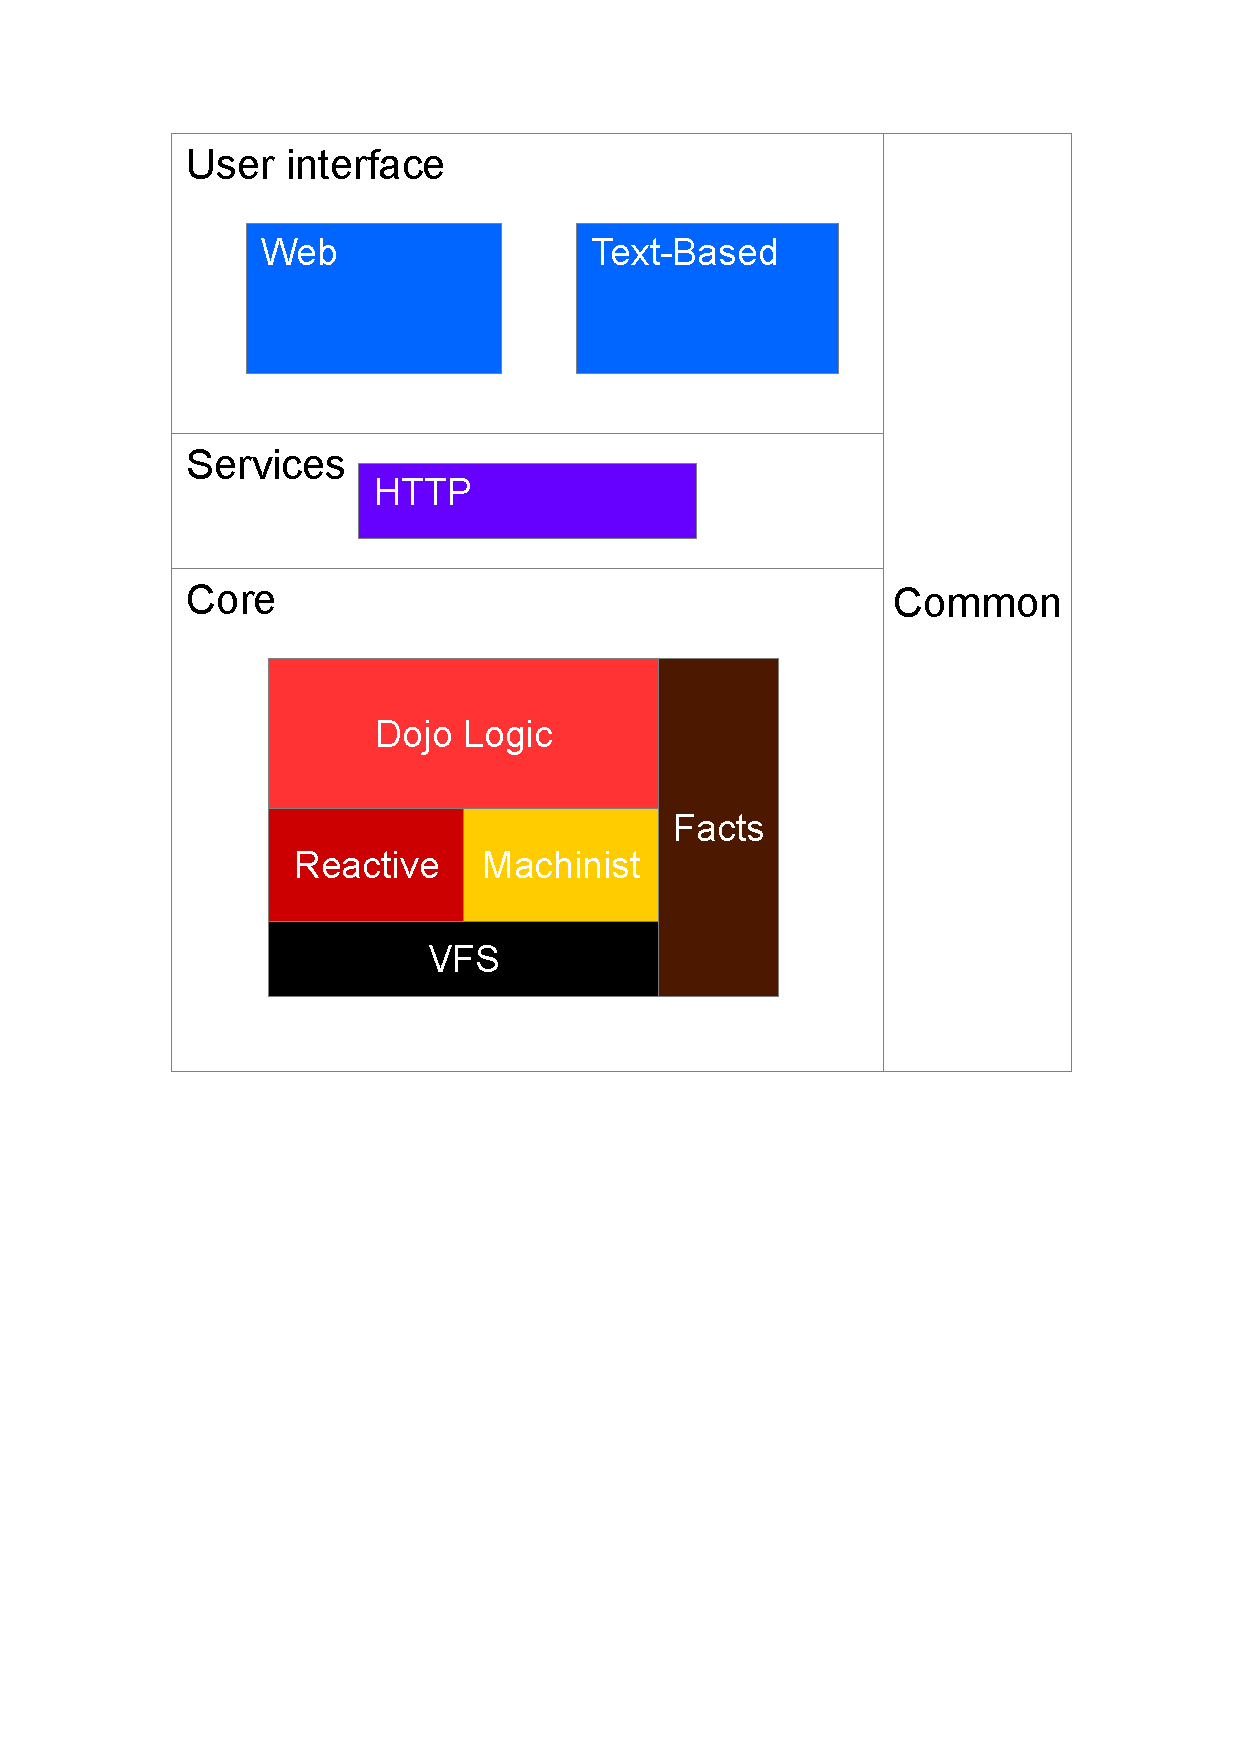
\includegraphics[width=\textwidth,  trim=2cm 12cm 2cm 1cm]{UML_figure/packages/general/DP_General.pdf}
				\caption{Diagram package : Overview}
			\end{center}
	\end{figure}
	\newpage
	\subsection{User Interface}
		This package provides user interface components that only rely on the public services exposed by the core system.
		\subsubsection{Web}
			This package contains the web user interface accessible through a web browser.
		\subsubsection{Text-based}
			This package contains the text-based user interface.\\
			This interface is meant to interact with unix-like batch tools.
	\subsection{HTTP}
		This package provides the web services which allow user interfaces to communicate with the core.
	\subsection{Core}
		This package provides the core features of the system i.e. the dojo logic and the infrastructure to make it works.
		\subsubsection{Dojo Logic}
			This package provides the business logic of online teaching.
		\subsubsection{Machinist}
			This package provides modules which manage sandboxed execution environments.
		\subsubsection{Reactive}
			This package provides modules for data update through dependencies.
		\subsubsection{VFS}
			This package provides modules implementing a versioned file system, that is a file system that remembers all its states.
		\subsubsection{Facts}
			This package provides request for data analysis.
	\subsection{Common}
		This package provides utilities useful to all the layers of the system.
%end chapter diagram package
